\immediate\write18{tex calligraphy.dtx}
\immediate\write18{tex spath.dtx}
\documentclass{article}
\usepackage{tikz}
\usepackage{calligraphy}
\usetikzlibrary{decorations.pathreplacing,matrix}

\begin{document}
\begin{tikzpicture}[line width=2pt]
\pen (0,0) -- ++(.5,.5) ++(.5,.5);
\end{tikzpicture}
\calligraphystyle{process pen=default}

\begin{tikzpicture}
\useasboundingbox (-3,-1) rectangle (3,2);
\calligraphy[annotate,annotation style={dashed,->,thin},annotation node style={2}{circle,draw,fill=white},heavy,pen colour=red,pen nib={1}{pen colour=green}] (0,0) .. controls +(45:1) and +(-135:1) .. +(3,0) [calligraphy,line style={light,pen nib={1}{pen colour=yellow}}] ++(1.5,0) .. controls +(-135:2) and +(45:2) .. +(0,-3) [calligraphy,line style={heavy}]  (0,-3) .. controls +(45:1) and +(-135:1) .. +(3,0) [calligraphy,line style={light}];
\end{tikzpicture}

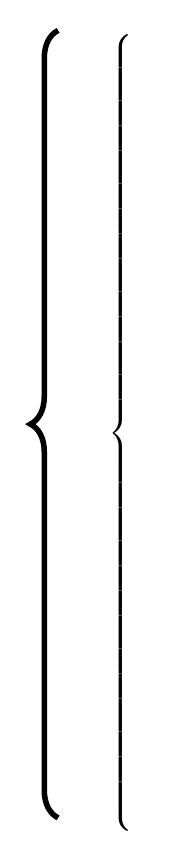
\begin{tikzpicture}
\pen (0,0);
\calligraphystyle{process pen=default}
\calligraphy[heavy] (0,0) .. controls +(-135:.05) and +(0,.3) .. ++(-.2,-.4) -- ++(0,-4.2) .. controls +(0,-.3) and +(45:.05) .. ++(-.2,-.4) ++(0,0) .. controls  +(-45:.05) and +(0,.3) .. ++(.2,-.4) -- ++(0,-4.2) .. controls +(0,-.3) and +(135:.05) .. ++(.2,-.4);
\draw[line width=2pt,decorate,decoration={brace,amplitude=10}] (1,-10) -- ++(0,10);
\node[anchor=north west,text height=10cm,outer sep=0pt,left delimiter=\{] (a) at (2,0) {};
\end{tikzpicture}

\begin{tikzpicture}
\pen (0,0);
\calligraphystyle{process pen=default,heavy line width=3mm}
\calligraphy[heavy, taper=end] (0,0) -- +(10,0);
\calligraphy[heavy, taper=start] (0,-1) -- +(10,0);
\end{tikzpicture}
\end{document}


\begin{tikzpicture}
\pen (-135:.25) -- (45:.25);
\draw[line width=.5cm] (0,0) .. controls +(45:1) and +(-135:1) .. ++(3,0);
\calligraphy (0,-1) .. controls +(45:1) and +(-135:1) .. ++(3,0);
\end{tikzpicture}

\begin{tikzpicture}[line width=2pt]
\pen (0,0);
\calligraphy[heavy,taper=end] (0,0) .. controls +(45:1) and +(-135:1) .. +(3,0) ++(1.5,0) .. controls +(-135:2) and +(45:2) .. +(0,-3)  (0,-3) .. controls +(45:1) and +(-135:1) .. +(3,0);
\calligraphy[light] (4,0) .. controls +(45:1) and +(-135:1) .. +(3,0) ++(1.5,0) .. controls +(-135:2) and +(45:2) .. +(0,-3)  (4,-3) .. controls +(45:1) and +(-135:1) .. +(3,0);
\end{tikzpicture}

\begin{tikzpicture}[line width=1pt]
\pen (-135:.125) -- (0,0) (45:.125);
\calligraphy[annotate] (0,0) .. controls +(45:1) and +(-135:1) .. +(3,0) ++(1.5,0) .. controls +(-135:2) and +(45:2) .. +(0,-3)  (0,-3) .. controls +(45:1) and +(-135:1) .. +(3,0);
\end{tikzpicture}


\begin{tikzpicture}[thick]
%\pen (0,0);
\coordinate (a) at (0,.5);
\coordinate (b) at (.5,0);
\coordinate (c) at (0,-.5);
\coordinate (d) at (-.5,0);
\draw (d) to[bend left] (c) to[out=150,in=210] (c);
\end{tikzpicture}

\end{document}

% Local Variables:
% tex-output-type: "pdf18"
% End: